\documentclass[a4paper,12pt]{article}
\usepackage{amsmath}
\usepackage{amssymb}
\usepackage[polish]{babel}
\usepackage{polski}
\usepackage[utf8]{inputenc}
\usepackage{geometry}
\usepackage[pdftex]{color,graphicx}
\usepackage{setspace}
\usepackage{wrapfig}
\usepackage{listings}
\usepackage{datetime}
\usepackage{indentfirst}
\renewcommand{\onehalfspacing}{\setstretch{1.6}}
\renewcommand{\dateseparator}{-}

\geometry{tmargin=2.5cm,bmargin=2.5cm,lmargin=2.5cm,rmargin=2.5cm}
\setlength{\parindent}{1cm}
\setlength{\parskip}{0mm}

\definecolor{lbcolor}{rgb}{0.95,0.95,0.95}
\lstset{
    backgroundcolor=\color{lbcolor},
    tabsize=4,
  language=C++,
  captionpos=b,
  tabsize=3,
  frame=lines,
  numbers=left,
  numberstyle=\tiny,
  numbersep=5pt,
  breaklines=true,
  showstringspaces=false,
  basicstyle=\footnotesize,
  identifierstyle=\color{magenta},
  keywordstyle=\color[rgb]{0,0,1},
  commentstyle=\color{green},
  stringstyle=\color{red}
  }
\newcommand{\linia}{\rule{\linewidth}{0.4mm}}
\begin{document}
	\begin{titlepage}
	\begin{center}
	
	\textsc{\LARGE Programowanie równoległe i rozproszone}\\[1.5cm]
	\linia\newline
	\textsc{\Large Projekt}\\[0.5cm]
	{ \huge \bfseries Algorytm RSA z wykorzystaniem OpenMP i CUDA \\[0.4cm] }
	\linia\newline

		\noindent
		\begin{minipage}{0.4\textwidth}
		\begin{flushleft} \large
		\emph{Autorzy:}\\
		Kordian \textsc{Kurdziel}\\Mateusz \textsc{Maciejak} 
		\end{flushleft}
		\end{minipage}

	\vfill

	\end{center}
	\end{titlepage}
\newpage
\section*{Wstęp}

Zrównoleglanie obliczeń jest, przy obecnej architekturze wieloprocesorowych komputerów sprawą niezmiernie istotną. Rozdzielenie zadań na kilka współbieżnie przetwarzanych bloków pozwala na uzyskanie znacznego przyśpieszenia wszelkiego rodzaju obliczeń i operacji wymagających mocy obliczeniowej. Na rynku istnieje wiele technologii pozwalających na tworzenie oprogramowania działającego współbieżnie. Do tego celu wykorzystują różne podejścia. Message Passing Interface (MPI) wykorzystuje procesy procesora do podziału zadań, Open Multi-Processing (OpenMp) wykorzystuje wątki a technologia Compute Unified Device Architecture (CUDA) korzysta z ogromnej mocy obliczeniowej zawartej w kartach nVidia.
    W naszym projekcie w celu porównania technologii działających na różnym sprzęcie postanowiliśmy sprawdzić sposób i wydajność zrównoleglania obliczeń poprzez podział zadań między wątki procesora (OpenMp) lub wątki karty graficznej (CUDA). Dokument ten stanowi formę dokumentacji do projektu zaliczeniowego oraz zawiera wysnute przez nas wnioski i obserwacje na temat badanych technologii w przypadku szyfrowania algorytmem RSA.


\section*{1 Cel projektu}

Celem projektu było zaimplementowanie algorytmu kryptograficznego jakim jest RSA z wykorzystaniem dwóch technologii OpenMP oraz CUDA. Jako punkt obserwacji został wybrany proces enkrypcji wiadomości, który jest długotrwały i w teorii powinien pozwolić się dobrze zrównoleglić. Dzięki zastosowaniu wyżej wymienionych technik zrównoleglania, oczekujemy że czas szyfrowania wiadomości ulegnie znacznej poprawie i zaobserwujemy ten proces w naszych rezultatach.

\section*{2 Algorytm RSA}

Jeden z pierwszych i obecnie najpopularniejszych asymetrycznych algorytmów kryptograficznych z kluczem publicznym, zaprojektowany w 1977 przez Rona Rivesta, Adi Shamira oraz Leonarda Adlemana. Pierwszy algorytm, który może być stosowany zarówno do szyfrowania jak i do podpisów cyfrowych. Bezpieczeństwo szyfrowania opiera się na trudności faktoryzacji dużych liczb złożonych. Jego nazwa pochodzi od pierwszych liter nazwisk jego twórców.

\textbf{Algorytm RSA składa się z trzech podstawowych kroków:}

1. Generacja klucza publicznego i tajnego. Klucz publiczny jest przekazywany wszystkim zainteresowanym i umożliwia zaszyfrowanie danych. Klucz tajny umożliwia rozszyfrowanie danych zakodowanych kluczem publicznym. Jest trzymany w ścisłej tajemnicy.
2. Użytkownik po otrzymaniu klucza publicznego, np. poprzez sieć Internet, koduje za jego pomocą swoje dane i przesyła je w postaci szyfru RSA do adresata dysponującego kluczem tajnym, np. do banku, firmy komercyjnej, tajnych służb. Klucz publiczny nie musi być chroniony, ponieważ nie umożliwia on rozszyfrowania informacji – proces szyfrowania nie jest odwracalny przy pomocy tego klucza. Zatem nie ma potrzeby jego ochrony i może on być powierzany wszystkim zainteresowanym bez ryzyka złamania kodu.

3. Adresat po otrzymaniu zaszyfrowanej wiadomości rozszyfrowuje ją za pomocą klucza tajnego.

Szyfrowanie odbywa się za pomocą klucza publicznego (n, e). Wiadomość musi zostać podzielona na części, a następnie każda część powinna zostać zmieniona na liczbę (która musi być większa od 0 i mniejsza niż n). W praktyce dzieli się wiadomość na fragmenty, z których każdy składa się z określonej ilości bitów.

Następnie każda liczba wchodząca w skład wiadomości jest podnoszona modulo n do potęgi równej e:
    ci = mie  (mod n)

Algorytmu RSA można użyć wielokrotnie (przy zastosowaniu różnych kluczy) do zaszyfrowania danej wiadomości, a następnie odszyfrować ją w dowolnej kolejności. Otrzymany wynik będzie zawsze taki sam, bez względu na kolejność operacji. Jednakże, nie należy szyfrować w ten sposób wiadomości więcej niż dwa razy, ponieważ ujawniają się wtedy podatności na ataki oparte na chińskim twierdzeniu o resztach.

Szyfrowanie może zostać przeprowadzone również przy użyciu klucza prywatnego. Cała procedura jest identyczna do opisanej powyżej, z różnicą, że do szyfrowania trzeba będzie użyć klucza prywatnego (n, d). Natomiast odbiorca wiadomości będzie musiał użyć odpowiadającego mu klucza publicznego, w celu odszyfrowania wiadomości.
 

\newpage
\section*{3 Metody zrównoleglenia algorytmu}

\subsection*{3.1 MPI - OpenMP - Open Multi-Processing}

Wieloplatformowy interfejs programowania aplikacji (API) umożliwiający tworzenie programów komputerowych dla systemów wieloprocesorowych z pamięcią dzieloną. Może być wykorzystywany w językach programowania C, C++ i Fortran na wielu architekturach, m.in. Unix i Microsoft Windows. Składa się ze zbioru dyrektyw kompilatora, bibliotek oraz zmiennych środowiskowych mających wpływ na sposób wykonywania się programu.

    Dzięki temu, że standard OpenMP został uzgodniony przez głównych producentów sprzętu i oprogramowania komputerowego, charakteryzuje się on przenośnością, skalowalnością, elastycznością i prostotą użycia. Dlatego może być stosowany do tworzenia aplikacji równoległych dla różnych platform, od komputerów klasy PC po superkomputery.

    OpenMP można stosować do tworzenia aplikacji równoległych działających na wieloprocesorowych węzłach klastrów komputerowych. W tym przypadku stosuje się rozwiązanie hybrydowe, w którym programy są uruchamiane na klastrach komputerowych pod kontrolą alternatywnego interfejsu MPI, natomiast do zrównoleglenia pracy węzłów klastrów wykorzystuje się OpenMP. Alternatywny sposób polegał na zastosowaniu specjalnych rozszerzeń OpenMP dla systemów pozbawionych pamięci współdzielonej (np. Cluster OpenMP Intela).


\subsection*{3.2 CUDA - Compute Unified Device Architecture}

Opracowana przez firmę Nvidia uniwersalna architektura procesorów wielordzeniowych (głównie kart graficznych) umożliwiająca wykorzystanie ich mocy obliczeniowej do rozwiązywania ogólnych problemów numerycznych w sposób wydajniejszy niż w tradycyjnych, sekwencyjnych procesorach ogólnego zastosowania.

Integralną częścią architektury CUDA jest oparte na języku programowania C środowisko programistyczne wysokiego poziomu, w którego skład wchodzą m.in. specjalny kompilator (nvcc), debugger (cuda-gdb, który jest rozszerzoną wersją debuggera gdb umożliwiającą śledzenie zarówno kodu wykonywanego na CPU, jak i na karcie graficznej), profiler oraz interfejs programowania aplikacji. Dostępne są również biblioteki, które można wykorzystać w językach Python, Fortran, Java oraz Matlab. Pierwsze wydanie środowiska współpracowało z systemami operacyjnymi Windows oraz Linux. Od wersji 2.0 działa również z Mac OS X.


\newpage
\section*{4 Opis programów}

W celu zaobserwowania przyśpieszenia i zbadania czasu potrzebnego do zaszyfrowania wiadomości w badanych przypadkach, zostały zaimplementowane dwa programy realizujące ten sam cel. Większość kodu związanego ściśle z algorytmem pozostaje taka sama, jednak różnice w obu technologiach i inne procesy kompilacji zmusiły nas do stworzenia dwóch zupełnie oddzielnych programów z powtarzającą się logiką. Wszystkie procesy, ważniejsze funkcje w programach oraz kody źródłowe zostały opisane w poniższej sekcji.

Kod prezentujący funkcję enkrypcji wiadomości:
\begin{lstlisting}
int encrypt(long int* in, long int exp, long int mod, long int* out, size_t len)
{
  for (int i=0; i < len; i++)
  {
     long int c = in[i];
     for (int z=1;z<exp;z++)
     {
        c *= in[i];
        c %= mod;
     }
     out[i] = c;
  }
  out[len]='\0';
  return 0;
}

\end{lstlisting}

Powyższy kod źródłowy zawiera wspólną dla obu technologii implementację szyfrowania wiadomości. Funkcja jako parametry przyjmuje wiadomość przekształconą na ciąg liczb typu long, referencje do dwóch zmiennych przechowujących wynik przekształceń podczas generowania klucza publicznego, wskaźnik do bufora przechowującego długość wyjściowej wiadomości oraz parametr określający długość wiadomości przeznaczonej do zaszyfrowania.

Funkcje obliczające klucz publiczny i prywatny prezentują się następująco:
\begin{lstlisting}
int publickey(long int p, long int q, long int *exp, long int *mod)
{

  *mod = (p-1)*(q-1);
  *exp = (int)sqrt(*mod);
  while (1!=gcd(*exp,*mod)) 
  {
     (*exp)++;
  }
  *mod = p*q;
  return 0;
}

int privatekey(long int p, long int q, long int pubexp, long int *exp, long int *mod)
{
  *mod = (p-1)*(q-1);
  *exp = 1;
  long int tmp=pubexp;
  while(1!=tmp%*mod)
  {
     tmp+=pubexp;
     tmp%=*mod;
     (*exp)++;
  }
  *mod = p*q;
  return 0;
}


\end{lstlisting}
W kolejnych linijkach postaramy się przedstawić cechy charakterystyczne dla obu testowanych technologii do zrównoleglania obliczeń.

\subsubsection*{4.1 OpenMP}

Technologia OpenMp zyskała wielu zwolenników ze względu na bardzo niski koszt wprowadzenia jej do już istniejącego kodu. Aby zrównoleglić pętlę, wystarczy dodać przed nią odpowiednie klauzule charakterystyczne dla tej technologii. Na poniższym fragmencie kodu można zobaczyć jak w nieznacznym stopniu uległ zmianie kod funkcji szyfrowania.


\begin{lstlisting}
int encrypt(long int* in, long int exp, long int mod, long int* out, size_t len)
{
  #pragma omp parallel for schedule(dynamic) num_threads(numberOfThreads)
  for (int i=0; i < len; i++)
  {
     long int c = in[i];
     for (int z=1;z<exp;z++)
     {
        c *= in[i];
        c %= mod;
     }
     out[i] = c;
  }
  out[len]='\0';
  return 0;
}

\end{lstlisting}


\subsubsection*{4.2 Cuda}

Technologia CUDA jest z pewnością dużo bardziej inwazyjna w już istniejący kod napisany przez programistę. Wymaga dodania specjalnych słów kluczowych przy każdej z metod, które mają być wykonane na karcie graficznej. Konieczne jest również kontrolowanie przez programistę, jakie zmienne są przechowywane w pamięci działającej na hoście a jakie na karcie graficznej. Z pewnością przejście z już istniejącego kodu do takiego, który można uruchomić współbieżnie na kartach z rodziny nVidia wymaga dużego narzutu na zmiany. W zamian technologia CUDA oferuje, bardzo często dużo większe przyśpieszenie obliczeń niż jest to możliwe na powszechnie wykorzystywanych procesorach.


\begin{lstlisting}
int encrypt(long int* in, long int exp, long int mod, long int* out, size_t len)
//Encrypt an array of long ints
//exp and mod should be the public key pair
//Each number, c', is decrypted by
// c = (c'^exp)%mod
{
  long int *d_inout;
  //Allocate memory in the separate memory space of the GPU
  cudaMalloc(&d_inout, sizeof(long int)*len);

  //copy data to the GPU
  cudaMemcpy(d_inout, in, sizeof(long int)*len, cudaMemcpyHostToDevice); //copy to GPU

   float time;
   cudaEvent_t start, stop;
    cudaEventCreate(&start);
    cudaEventCreate(&stop);
    cudaEventRecord(start, 0);

  //Launch the kernel on the GPU with 1024 threads arranged in blocks of size BLOCKWID
  decrypt_kernel<<<BLOCK_SIZE, GRID_SIZE>>> (d_inout, exp, mod, len);

   //End timer and put result into time variable
   cudaDeviceSynchronize();             
    cudaEventRecord(stop, 0);
    cudaEventSynchronize(stop);
    cudaEventElapsedTime(&time, start, stop);

   printf("%.4f\n", time);

  //copy data back from GPU
  cudaMemcpy(out, d_inout, sizeof(long int)*len, cudaMemcpyDeviceToHost); //copy from GPU

  out[len]=0; //Terminate with a zero
  cudaFree(d_inout);
  return 0;
}

\end{lstlisting}

Powyższy fragment przedstawia funkcję wywoływaną z głównej metody. Jak możemy zauważyć, programista musi zaalokować pamięć na urządzeniu z wykorzystaniem oferowanych przez technologię CUDA funkcji. Przedstawione wyżej metody są dostępne tylko i wyłącznie wtedy gdy program uruchamiany jest na sprzęcie wyposażonym w kartę nVidia, co stanowi spore ograniczenie i zmusza do przemyślanego definiowania takich funkcji. Jak możemy zauważyć oryginalny kod algorytmu szyfrowania musiał ulec znaczącym zmianom by mógł być uruchomiony na karcie graficznej. 
Logika szyfrowania została  rozbita na funkcję uruchamianą na karcie graficznej. Specjalna klauzula \textbf{global} informuje kompilator, że funkcja jest tak zwanym kernelem i zostanie uruchomiona na urządzeniu. Wywoływana jest wykorzystując specjalną sementykę technologii CUDA. W poniższych fragmentach prezentujemy kod uruchamiany na karcie graficznej.


\begin{lstlisting}
__global__ void decrypt_kernel(long int* inout, long int exp, long int mod, size_t len)
{
  for (int t = threadIdx.x + blockIdx.x*blockDim.x; t<len ;t+=blockDim.x*gridDim.x)
  {
     if (t<len) inout[t] = fastexp(inout[t], exp, mod);
  }

#ifdef __CUDA
__device__ __host__
#endif
long int fastexp(long int base, long int exp, long int mod)
{
  long int out = 1;
  while(exp>0)
  {
     if(1==exp%2)
     {
        out*=base;
        out%=mod;
     } 
     base=base*base;
     base%=mod;
     exp/=2;
  }
  return out;
}

\end{lstlisting}

Klauzula \textbf{device} oznacza, że funkcja jest wywoływana z karty graficznej a nie z programu głównego. Dodatkowo funkcja ta też została opatrzona klauzulą \textbf{host} gdyż w przypadku braku karty nVidia w komputerze na którym uruchamiany jest problem prezentowana funkcja uruchamiana jest w tradycyjny sposób z wykorzystaniem mocy obliczeniowej jednostki CPU.

\newpage


\section*{5 Pomiary}

\subsection*{5.1 OpenMP}

Poniższe wykresy i tabela z wynikami, przedstawiające zależność czasową oraz przyspieszenia zostały oparte na średnich wynikach programu uruchamianych lokalnie na maszynie wirtualnej. Wykorzystany został 6 rdzeniowy procesor Intel z technologią Hyperthreadingu.

\begin{figure}[!ht]
	\centering
  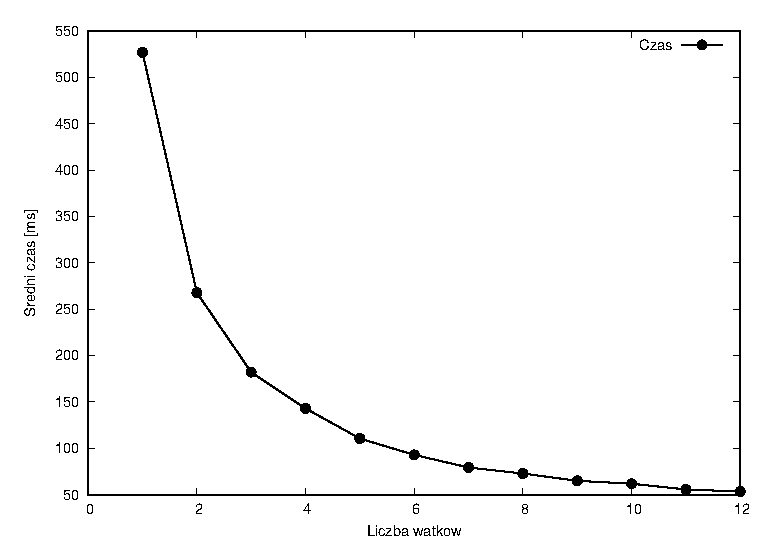
\includegraphics[width=0.7\textwidth]{openMPWykresCzas.eps}
  \caption{Wykres zależności czasu wykonywania obliczeń od liczby wątków}
\end{figure}

\begin{figure}[!ht]
	\centering
  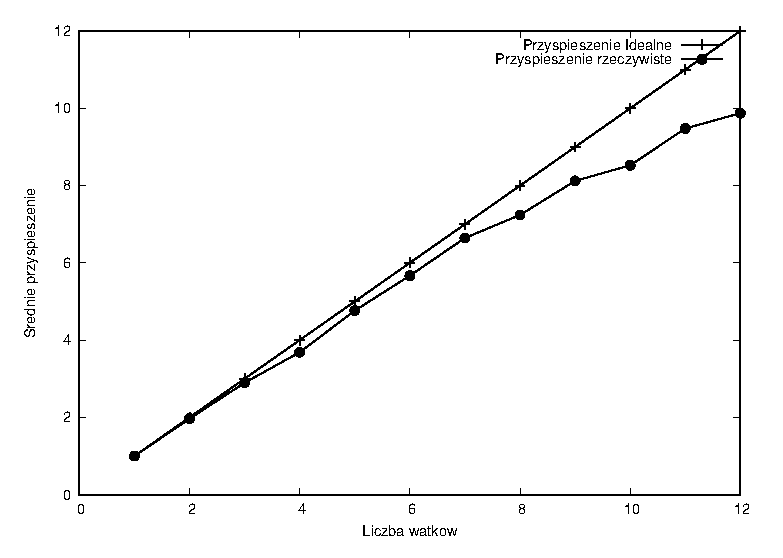
\includegraphics[width=0.7\textwidth]{openMPWykresPrzyspieszenie.eps}
  \caption{Wykres przyspieszenia działania programu w zależności od liczby wątków}
\end{figure}

\newpage
\begin{table}[htb]
\centering
\begin{tabular}{|c|c|c|}\hline
Liczba wątków OpenMP & Czas[ms] & Przyspieszenie\\ \hline 
1 & 526.98 & 1.00\\ \hline 
2 & 267.85 & 1.96\\ \hline 
3 & 182.06 & 2.89\\ \hline 
4 & 143.019 & 3.68\\ \hline 
5 & 110.60 & 4.76\\ \hline 
6 & 92.95 & 5.66\\ \hline 
7 & 79.34 & 6.64\\ \hline 
8 & 72.80 & 7.23\\ \hline
9 & 64.90 & 8.11\\ \hline 
10 & 61.82 & 8.52\\ \hline 
11 & 55.61 & 9.47\\ \hline 
12 & 53.37 & 9.87\\ \hline
\end{tabular}
\end{table}

Jak widać dzięki zastosowaniu technologii OpenMP, wykorzystując dostępne wątki, udało się znacząco przyspieszyć wykonywanie programu. Uzyskane rzeczywiste przyspieszenie jest bliskie idealnemu, co może świadczyć o tym, że powyższa klasa problemów nadaje się całkiem dobrze do wykorzystywania obliczeń wielowątkowych.
Jak można zauważyć na wykresie przyspieszenie działania programu wzrastało wraz z liczbą wykorzystywanych wątków nawet po przekroczeniu granicy jednostek fizycznych. Potem wraz ze wzrostem liczby wątków program dalej wykazywał przyspieszenie. Można więc wyciągnąć wniosek, że technologia Hyperthreadingu, wykorzystywana w procesorach Intela, działa aż tak wydajnie przy takich obliczeniach.
\newpage

\subsection*{5.2 CUDA}
Poniższe wykresy i tabela przedstawia wyniki uzyskane na serwerze CUDA. Czas obliczeń dla każdej ilości bloków przedstawionej na wykresie został przetestowany 5 razy a z wyników wyciągnięto średnią arytmetyczną.


\begin{figure}[!ht]
	\centering
  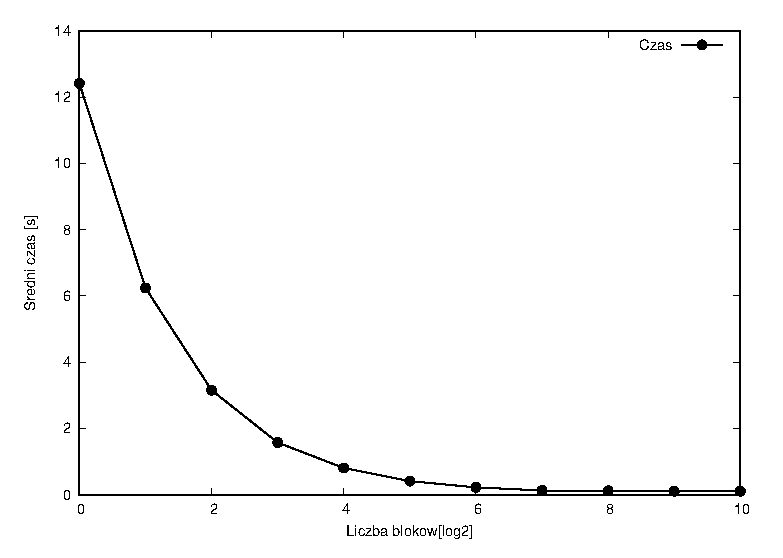
\includegraphics[width=0.7\textwidth]{cudaWykresCzas.eps}
  \caption{Wykres zależności czasu wykonywania obliczeń od liczby bloków}
\end{figure}

\begin{figure}[!ht]
	\centering
  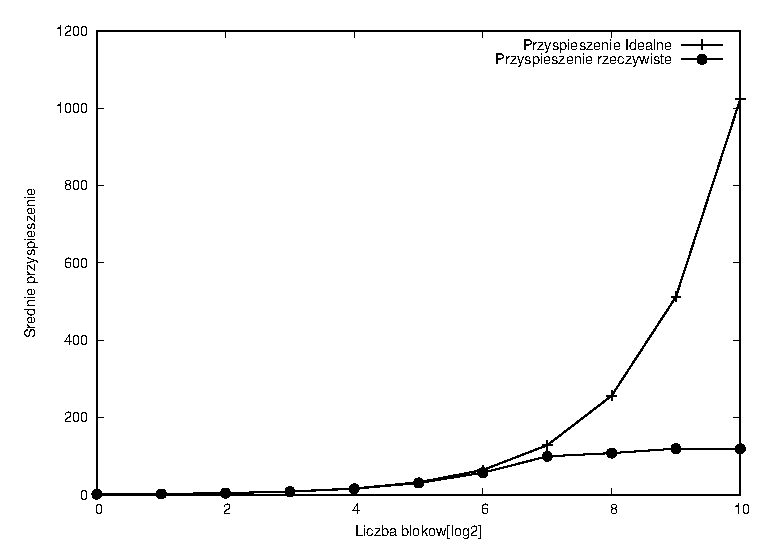
\includegraphics[width=0.7\textwidth]{cudaWykresPrzyspieszenie.eps}
  \caption{Wykres zależności przyspieszenia od liczby bloków}
\end{figure}

\newpage
\begin{table}[htb]
\centering
\begin{tabular}{|c|c|c|}\hline
Liczba bloków CUDA & Czas[s] & Przyspieszenie\\\hline 
1 & 12.41 & 1.00\\ \hline 
2 & 6.24 & 1.99\\ \hline 
4 & 3.15 & 3.93\\ \hline 
8 & 1.57 & 7.89\\ \hline 
16 & .80 & 15.44\\ \hline 
32 & .41 & 30.27\\ \hline 
64 & .21 & 56.79\\ \hline 
128 & .12 & 99.23\\ \hline
256 & .11 & 107.52\\ \hline 
512 & .10 & 119.26\\ \hline 
1024 & .10 & 118.67\\ \hline 
\end{tabular}
\end{table}
Jak można zauważyć, czas obliczeń znacząco się zmniejsza wraz z rozpoczęciem zwiększania liczby bloków. Wraz z wzrostem liczby bloków różnice pomiędzy sąsiednimi czasami stają się coraz mniejsze. 

\clearpage
\section*{6 Wnioski}

	

\end{document}
